\documentclass[tikz, border=4pt]{standalone}
\usepackage{amsmath}
\usetikzlibrary{arrows.meta, decorations.pathreplacing}

% ---- color definitions ----
\definecolor{suOneColor}{RGB}{31, 119, 180}   % blue
\definecolor{suTwoColor}{RGB}{214, 94, 37}    % orange

\begin{document}
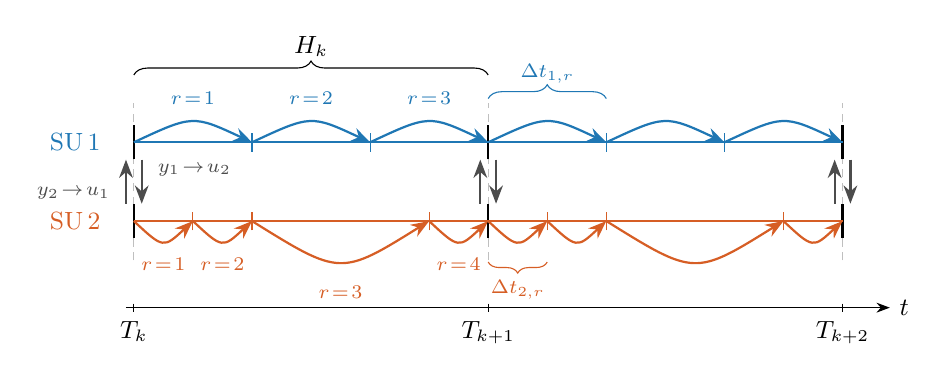
\begin{tikzpicture}[
    >=Stealth,
    su line/.style={thick},
    comm line/.style={densely dashed, gray!50},
    comm tick/.style={thick},
    brace above/.style={decorate,
        decoration={brace, amplitude=5pt, raise=3pt}},
    brace below/.style={decorate,
        decoration={brace, amplitude=4pt, raise=2pt, mirror}},
]

% ---- layout parameters ----
\def\H{4.5}         % macro step width (cm)
\def\nMacro{2}      % number of macro steps
\def\yOne{1}      % y of SU 1
\def\yTwo{0}        % y of SU 2
\def\tk{0.12}       % tick half-height
\def\arcH{0.35}     % arc height

\pgfmathsetmacro{\xEnd}{\nMacro*\H}

% ---- time axis ----
\draw[->] (-0.1, -1.1) -- (\xEnd+0.6, -1.1)
    node[right, font=\small] {$t$};

% ---- communication point grid ----
\foreach \k in {0,...,\nMacro} {
    \pgfmathsetmacro{\xk}{\k*\H}
    \draw[comm line] (\xk, \yTwo-0.5) -- (\xk, \yOne+0.5);
    \draw[comm tick] (\xk, \yOne-\tk*1.8) -- (\xk, \yOne+\tk*1.8);
    \draw[comm tick] (\xk, \yTwo-\tk*1.8) -- (\xk, \yTwo+\tk*1.8);
    \draw (\xk, -1.05) -- (\xk, -1.15);
}
% communication point labels
\node[below, font=\small] at (0, -1.15)       {$T_k$};
\node[below, font=\small] at (\H, -1.15)      {$T_{k+1}$};
\node[below, font=\small] at (2*\H, -1.15)    {$T_{k+2}$};

% ======== SU 1 (blue) ========
\draw[su line, suOneColor] (0, \yOne) -- (\xEnd, \yOne);
\node[left, font=\small, suOneColor] at (-0.3, \yOne) {SU\,$1$};

% SU 1: 3 internal steps per macro step → arcs above the line
\foreach \k in {0,...,1} {
    \foreach \s in {0,...,2} {
        \pgfmathsetmacro{\xL}{\k*\H + \s*\H/3}
        \pgfmathsetmacro{\xR}{\k*\H + (\s+1)*\H/3}
        \pgfmathsetmacro{\xM}{(\xL+\xR)/2}
        % arc
        \draw[suOneColor, thick, ->]
            (\xL, \yOne) .. controls (\xM, \yOne+\arcH) .. (\xR, \yOne);
    }
}

% SU 1 micro step tick marks (interior only)
\foreach \k in {0,...,1} {
    \foreach \s in {1,...,2} {
        \pgfmathsetmacro{\xpos}{\k*\H + \s*\H/3}
        \draw[suOneColor] (\xpos, \yOne-\tk) -- (\xpos, \yOne+\tk);
    }
}

% SU 1: r labels on first macro step arcs
\node[above, font=\scriptsize, suOneColor] at ({0*\H + 1*\H/6}, \yOne+\arcH)
    {$r\!=\!1$};
\node[above, font=\scriptsize, suOneColor] at ({0*\H + 3*\H/6}, \yOne+\arcH)
    {$r\!=\!2$};
\node[above, font=\scriptsize, suOneColor] at ({0*\H + 5*\H/6}, \yOne+\arcH)
    {$r\!=\!3$};

% ======== SU 2 (orange) — adaptive internal steps ========
\draw[su line, suTwoColor] (0, \yTwo) -- (\xEnd, \yTwo);
\node[left, font=\small, suTwoColor] at (-0.3, \yTwo) {SU\,$2$};

% SU 2: 4 non-uniform internal steps per macro step
% Step boundaries as fractions of H: 0, 1/6, 2/6, 5/6, 1
% r=1: 1/6 H,  r=2: 1/6 H,  r=3: 3/6 H (large),  r=4: 1/6 H
\foreach \k in {0,...,1} {
    \pgfmathsetmacro{\base}{\k*\H}
    % r=1: [0, 1/6]
    \pgfmathsetmacro{\xL}{\base + 0}
    \pgfmathsetmacro{\xR}{\base + \H/6}
    \pgfmathsetmacro{\xM}{(\xL+\xR)/2}
    \draw[suTwoColor, thick, ->]
        (\xL, \yTwo) .. controls (\xM, \yTwo-\arcH) .. (\xR, \yTwo);
    % r=2: [1/6, 2/6]
    \pgfmathsetmacro{\xL}{\base + \H/6}
    \pgfmathsetmacro{\xR}{\base + 2*\H/6}
    \pgfmathsetmacro{\xM}{(\xL+\xR)/2}
    \draw[suTwoColor, thick, ->]
        (\xL, \yTwo) .. controls (\xM, \yTwo-\arcH) .. (\xR, \yTwo);
    % r=3: [2/6, 5/6] — large adaptive step
    \pgfmathsetmacro{\xL}{\base + 2*\H/6}
    \pgfmathsetmacro{\xR}{\base + 5*\H/6}
    \pgfmathsetmacro{\xM}{(\xL+\xR)/2}
    \draw[suTwoColor, thick, ->]
        (\xL, \yTwo) .. controls (\xM, \yTwo-0.7) .. (\xR, \yTwo);
    % r=4: [5/6, 1]
    \pgfmathsetmacro{\xL}{\base + 5*\H/6}
    \pgfmathsetmacro{\xR}{\base + \H}
    \pgfmathsetmacro{\xM}{(\xL+\xR)/2}
    \draw[suTwoColor, thick, ->]
        (\xL, \yTwo) .. controls (\xM, \yTwo-\arcH) .. (\xR, \yTwo);
}

% SU 2 micro step tick marks (interior boundaries: 1/6, 2/6, 5/6)
\foreach \k in {0,...,1} {
    \pgfmathsetmacro{\base}{\k*\H}
    \foreach \frac in {1, 2, 5} {
        \pgfmathsetmacro{\xpos}{\base + \frac*\H/6}
        \draw[suTwoColor] (\xpos, \yTwo-\tk) -- (\xpos, \yTwo+\tk);
    }
}

% SU 2: r labels on first macro step
\node[below, font=\scriptsize, suTwoColor]
    at ({1*\H/12}, \yTwo-\arcH) {$r\!=\!1$};
\node[below, font=\scriptsize, suTwoColor]
    at ({3*\H/12}, \yTwo-\arcH) {$r\!=\!2$};
\node[below, font=\scriptsize, suTwoColor]
    at ({7*\H/12}, \yTwo-0.7) {$r\!=\!3$};
\node[below, font=\scriptsize, suTwoColor]
    at ({11*\H/12}, \yTwo-\arcH) {$r\!=\!4$};


% ---- data exchange arrows at communication points ----
\foreach \k in {0,...,1} {
    \pgfmathsetmacro{\xk}{\k*\H}
    % y_1 → u_2  (downward, right offset)
    \draw[->, thick, black!70] (\xk+0.1, \yOne-0.22)
        -- (\xk+0.1, \yTwo+0.22);
    % y_2 → u_1  (upward, left offset)
    \draw[->, thick, black!70] (\xk-0.1, \yTwo+0.22)
        -- (\xk-0.1, \yOne-0.22);
}
% also at the last communication point
\draw[->, thick, black!70] (2*\H+0.1, \yOne-0.22)
    -- (2*\H+0.1, \yTwo+0.22);
\draw[->, thick, black!70] (2*\H-0.1, \yTwo+0.22)
    -- (2*\H-0.1, \yOne-0.22);

% ---- exchange labels (at first comm point) ----
\node[right, font=\scriptsize, black!70]
    at (0.18, {\yOne/2 + 0.15}) {$y_1 \!\to\! u_2$};
\node[left, font=\scriptsize, black!70]
    at (-0.18, {\yOne/2 - 0.15}) {$y_2 \!\to\! u_1$};

% ---- braces ----
% macro step H_k above everything
\draw[brace above] (0, \yOne+0.75)
    -- node[above=6pt, font=\small] {$H_k$}
    (\H, \yOne+0.75);

% micro step SU 1 (second macro step, less crowded than first with r labels)
\draw[brace above, suOneColor] (\H, \yOne+0.45)
    -- node[above=5pt, font=\scriptsize, suOneColor] {$\Delta t_{1,r}$}
    ({\H + \H/3}, \yOne+0.45);

% micro step SU 2 (second macro step)
\draw[brace below, suTwoColor] (\H, \yTwo-0.45)
    -- node[below=5pt, font=\scriptsize, suTwoColor] {$\Delta t_{2,r}$}
    ({\H + \H/6}, \yTwo-0.45);

\end{tikzpicture}
\end{document}
